These are working notes for the low density parameters in \maestro.
In low density regions, we modify the behavior of the algorithm.  Here
is a summary of some parameters, and a brief description of what they
do.
\begin{itemize}
\item \runparam{base\_cutoff\_density}, $\rho_{\rm base}$, (real):\\ \\
Essentially controls the lowest density allowed in the simulation and modifies the behavior
of several modules.
\item {\tt base\_cutoff\_density\_coord(:)} (integer array):\\ \\
For each level in the radial base state array, this is the coordinate of the first cell
where $\rho_0 < \rho_{\rm base}$.  Slightly more complicated for multilevel problems.

\item \runparam{anelastic\_cutoff}, $\rho_{\rm anelastic}$, (real):\\ \\
If $\rho_0 < \rho_{\rm anelastic}$, we modify the computation of $\beta_0$ in the
divergence constraint.

\item {\tt anelastic\_cutoff\_coord(:)} (integer array):\\ \\
Anelastic cutoff analogy of {\tt base\_cutoff\_density\_coord(:)}.

\item \runparam{burning\_cutoff\_density}, $\rho_{\rm burning}$,  (real):\\ \\
If $\rho < \rho_{\rm burning}$, don't call the burner in this cell.

\item {\tt burning\_cutoff\_density\_coord(:)} (integer array):\\ \\
Burning cutoff analogy of {\tt base\_cutoff\_density\_coord(:)}.

\item \runparam{buoyancy\_cutoff\_factor} (real):\\ \\
When computing velocity forcing, set the buoyance term ($\rho-\rho_0$) to 0 if 
$\rho < $ {\tt buoyancy\_cutoff\_factor} * {\tt base\_cutoff\_density}.

\item \runparam{do\_eos\_h\_above\_cutoff} (logical):\\ \\
If {\rm true}, at the end of the advection step, for each cell where 
$\rho < \rho_{\rm base}$, recompute $h = h(\rho,p_0,X)$.
\end{itemize}

\section{Computing the Cutoff Values}
We compute {\tt anelastic\_cutoff\_coord}(:), {\tt base\_cutoff\_density\_coord}(:), 
and {\tt burning\_cutoff\_density\_coord}(:) in analogous fashion.

\subsection{Single-Level Planar or any Spherical}
Here the base state exists as a single one-dimensional array with constant grid
spacing $\Delta r$.  Basically, we set the corresponding coordinate equal to $r$ as soon 
as $\rho_0(r)$ is less than  or equal to that particular cutoff value.
See Figure \ref{Fig:Cutoff} for a graphical representation.
%%%%%%%%%%%%%%%%%%%%%%%%%%%%%%%%%
\begin{figure}[hpb]
\centering
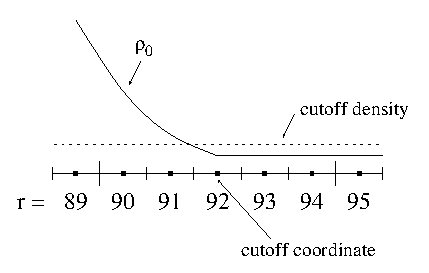
\includegraphics[width=4.0in]{\lodensfigpath/cutoff}\hspace{0.2in}
\caption[Cutoff density and coordinates]{Image of how the cutoff density and cutoff coordinates
are related for single-level planar and all spherical problems.}
\label{Fig:Cutoff}
\end{figure}
%%%%%%%%%%%%%%%%%%%%%%%%%%%%%%%%%

Note that for single-level planar or any spherical problem, saying
$r\ge$ {\tt anelastic\_cutoff\_coord} is analogous to saying
$\rho_0(r)\le$ \runparam{anelastic\_cutoff}.  Also, saying $r<$ {\tt
anelastic\_cutoff\_coord} is analogous to saying $\rho_0(r)>$ {\tt
anelastic\_cutoff}.  Ditto for \runparam{base\_cutoff\_density} and {\tt
base\_cutoff\_density\_coord}.

\subsection{Multilevel Planar}
In this case, the base state exists as several one-dimensional arrays, each with
different grid spacing.  Refer to Figure \ref{Fig:Cutoff_Multi} in the following examples.
The guiding principle is to check whether $\rho_0$ falls below $\rho_{\rm cutoff}$ on the finest
grid first.  If not, check the next coarser level.  Continue until you reach the base grid.
Some examples are in order:
%%%%%%%%%%%%%%%%%%%%%%%%%%%%%%%%%
\begin{figure}[hpb]
\centering
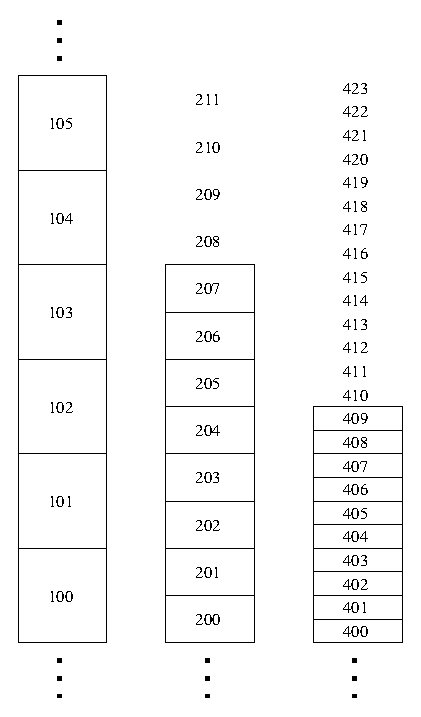
\includegraphics[width=2.0in]{\lodensfigpath/cutoff_multi}\hspace{0.2in}
\caption{Multilevel cutoff density example.}
\label{Fig:Cutoff_Multi}
\end{figure}
%%%%%%%%%%%%%%%%%%%%%%%%%%%%%%%%%

\begin{itemize}

\item {\bf Example 1:} $\rho_{0,104} > \rho_{\rm cutoff}$ and $\rho_{0,105} < \rho_{\rm cutoff}$.\\ \\
{\tt cutoff\_density\_coord}(1) = 105\\
{\tt cutoff\_density\_coord}(2) = 210\\
{\tt cutoff\_density\_coord}(3) = 420\\ \\
This is the simplest case in which the cutoff transition happens on the coarsest level.
In this case, the cutoff coordinates at the finer levels are simply propagated from the
coarsest level, even though they do not correspond to a valid region.

\item {\bf Example 2:} $\rho_{0,403} > \rho_{\rm cutoff}$ and $\rho_{0,404} < \rho_{\rm cutoff}$.\\ \\
{\tt cutoff\_density\_coord}(1) = 101\\
{\tt cutoff\_density\_coord}(2) = 202\\
{\tt cutoff\_density\_coord}(3) = 404\\ \\
In this case, the cutoff transition happens where the finest grid is present.  Happily, the
transition occurs at a location where there is a common grid boundary between all three levels.
Therefore, we simply propagate the cutoff density coordinate from the finest level downward.

\item {\bf Example 3:} $\rho_{0,404} > \rho_{\rm cutoff}$ and $\rho_{0,405} < \rho_{\rm cutoff}$.\\ \\
{\tt cutoff\_density\_coord}(1) = 102\\
{\tt cutoff\_density\_coord}(2) = 203\\
{\tt cutoff\_density\_coord}(3) = 405\\ \\
In this case, the cutoff transition happens where the finest grid is present.  However, the
transition occurs at a location where there NOT is a common grid boundary between all three 
levels.  We choose to define the cutoff transition at the coarser levels as being at the
corresponding boundary that is at a larger radius than the location on the finest grid.

\end{itemize}

Note: if $\rho_0$ does not fall below $\rho_{\rm cutoff}$ at any level, we set the cutoff 
coordinate at the fine level to be first first cell above the domain and propagate the 
coordinate to the coarser levels.

\section{When are the Cutoff Coordinates Updated?}

At several points in the algorithm, we compute {\tt anelastic\_cutoff\_coord}(:), 
{\tt base\_cutoff\_density\_coord}(:), and {\tt burning\_cutoff\_density\_coord}(:):

\begin{itemize}

\item After we call {\tt initialize} in {\tt varden}.

\item After reading the base state from a checkpoint file when restarting.

\item After regridding.

\item After advancing $\rho_0$ with {\tt advect\_base\_dens}.

\item After advancing $\rho$ and setting $\rho_0 = \overline{\rho}$.

\item At the beginning of the second-half of the algorithm ({\bf Step 6}), we reset
  the coordinates to the base-time values using $\rho_0^n$.

\end{itemize}

\section{Usage of Cutoff Densities}

\subsection{anelastic\_cutoff}\label{Sec:Anelastic Cutoff}

The \runparam{anelastic\_cutoff} is the density below which we modify the constraint.


\begin{itemize}

\item In {\tt probin}, {\tt anelastic\_cutoff} is set to $3\times 10^6$ by default.

\item In {\tt make\_div\_coeff}, for 
  $r \ge {\tt anelastic\_cutoff\_coord}$, we set
  ${\tt div\_coeff}(n,r) = {\tt div\_coeff}(n,r-1) * \rho_0(n,r)/\rho_0(n,r-1)$.

\item in {\tt make\_S}, we set {\tt delta\_gamma1\_term} and {\tt delta\_gamma1} 
  to zero for $r \ge {\tt anelastic\_cutoff\_coord}$.  This is only relevant
  if you are running with \runparam{use\_delta\_gamma1\_term} {\tt = T}.

\item Some versions of {\tt sponge}, use {\tt anelastic\_cutoff} in a problem dependent way.

\end{itemize}

\subsection{base\_cutoff\_density}\label{Sec:Base Cutoff Density}

The \runparam{base\_cutoff\_density} is the lowest density that we model.

\begin{itemize}

\item In {\tt probin}, {\tt base\_cutoff\_density} is set to $3\times 10^6$ by default.

\item In {\tt base\_state}, we compute a physical cutoff location,
  {\tt base\_cutoff\_density\_loc}, which is defined as the physical
  location of the first cell-center at the coarsest level for which
  $\rho_0 \le {\tt base\_cutoff\_density}$.  This is a trick used for making
  the data consistent for multiple level problems.  When we are generating the 
  initial background/base state, if we are above {\tt base\_cutoff\_density\_loc}, 
  just use the values for $\rho,T$, and $p$ at {\tt base\_cutoff\_density\_loc}.
  When we check whether we are in HSE, we use {\tt base\_cutoff\_density\_loc}.

\item In {\tt make\_S\_nodal}, {\tt make\_macrhs}, and {\tt make\_w0}, 
  we only add the volume discrepancy for $r < {\tt base\_cutoff\_density\_coord}$
  (in plane parallel) and if $\rho_0^{\rm cart} > {\tt base\_cutoff\_density}$ 
  (in spherical).

\item In {\tt mkrhohforce} for plane-parallel, for
  $r \ge {\tt base\_cutoff\_density\_coord}$, we
  compute $\nabla p_0$ with a difference stencil instead of simply
  setting it to $\rho_0 g$.

\item In {\tt update\_scal}, if $\rho \le {\tt base\_cutoff\_density}$
   and \runparam{do\_eos\_h\_above\_cutoff}, we call the EOS to compute $h$.

\item In {\tt update\_scal}, if $\rho \le {\tt base\_cutoff\_density}/2$
   we set it to ${\tt base\_cutoff\_density}/2$.

\item In {\tt make\_grav} for spherical, we only add the enclosed mass if
  $\rho_0 > {\tt base\_cutoff\_density}$.

\item In {\tt enforce\_HSE}, we set $p_0(r+1) = p_0(r)$ for 
  $r \ge {\tt base\_cutoff\_density\_coord}$.

\item In {\tt make\_psi} for plane-parallel, we only compute $\psi$ for 
  $r < {\tt base\_cutoff\_density\_coord}$.

\end{itemize}

\subsection{burning\_cutoff}

The burning cutoff determines where we call the reaction network to
get the nuclear energy generation rate and composition changes.  For
densities below the burning cutoff, we do not call the network.

\begin{itemize}

\item In {\tt probin}, \runparam{burning\_cutoff\_density} is set to 
  \runparam{base\_cutoff\_density}.  There is no option to set 
  {\tt burning\_cutoff\_density} using the inputs file.

\item In {\tt react\_state}, we only call the burner if 
  $\rho >$ {\tt burning\_cutoff\_density}.


\end{itemize}


\subsection{buoyancy\_cutoff\_factor}

The \runparam{buoyancy\_cutoff\_factor} is used to zero out the forcing terms
to the velocity equation at low densities.

\begin{itemize}

\item In {\tt init\_base\_state} we print out the value of the
   the density at which the buoyancy cutoff would take effect,
   {\tt buoyancy\_cutoff\_factor * base\_cutoff\_density}.

\item In {\tt mk\_vel\_force}, we zero out {\tt rhopert}, the
   perturbational density used in computing the buoyancy force,
   if $\rho < \mathtt{buoyancy\_cutoff\_factor * base\_cutoff\_density}$.

\item In {\tt mk\_vel\_force}, for spherical problems, we 
   zero out {\tt centrifugal\_term}, the centrifugal force for
   rotating stars, if $\rho < \mathtt{buoyancy\_cutoff\_factor *
   base\_cutoff\_density}$.

\item In {\tt make\_explicit\_thermal}, if \runparam{limit\_conductivity} {\tt = T}, then for 
$\rho < \mathtt{buoyancy\_cutoff\_factor}$ \\ $* \mathtt{base\_cutoff\_density}$, we
zero out the thermal coefficients, effectively turning off thermal
diffusion there.

\end{itemize}





